
%  \section{The PSF profile analysis}

Since the complex 6-parameter PSF fit given by Eq.~(\ref{eq:SDSSPSF}) was adopted by 
the SDSS processing pipeline, significant progress has been made in validating the 
\vk~model of the atmosphere and measuring the associated outer
scale (see, for example, \citealt{Tokovinin2002}, \citealt{Boccas2004}, and \citealt{MartinezMessenger}).
In this section, we describe our much simpler 2-parameter fits to the SDSS PSF
radial profiles using the \vk~atmosphere model.

The seeing profile predicted by the \vk~atmosphere model is a two-parameter
family that can be parametrized by the FWHM and the so-called outer scale
parameter. The Kolmogorov seeing profile is a special case of the 
\vk~seeing with the infinitely large outer scale. The radial profiles of the 
\vk~PSF with a few different values of outer scale are shown in Fig.~\ref{fig:vonK} (left). 


Our fitting of each PSF radial profile is a 2-step process. First we fit the
measured PSF profile to a \vk~PSF with only one free parameter -
the FWHM of the \vk~profile, while a fiducial outer scale of 30 meters
is assumed fixed. As discernible from Fig.~\ref{fig:vonK}, the impact of the exact
value of $L_0$ on the profile shape is small. A fixed value of $L_0$ induces a small 
systematic uncertainty in the normalization of the contribution of instrumental PSF, 
discussed in \S~\ref{sec:instrPSF}  below. The \vk~PSF profile is generated by creating 
the atmosphere structure function first, as given by Eq. (18) in \cite{Tokovinin2002},
then calculating the PSF through the Optical Transfer Function. 
Pixel integration is taken into account by a factor of 10 oversampling.

Ideally, the Fried parameter $r_0$ would be used as the free
parameter in the fit to the \vk~model. However, 
that would require us to calculate the special functions and do the
Fourier Transform on a large array for each function evaluation.
Instead, we opted to generate a single \vk~PSF template with the FWHM of 
1.0 arcsec. In our one-parameter \vk~fit, we only stretch or compress
the template radially to get the best match with the data, in the
least-square sense.
Fig.~\ref{fig:vonK} (right) shows a comparison of three PSF profiles,
one generated with FWHM of 1.0 arcsec, the other two generated with
FWHM of 0.5 and 2.0 arcsec, respectively, then stretched and
compressed to 1.0 arcsec. The three curves are seen to be almost
indistinguishable.

\begin{figure}[ht]
\centering
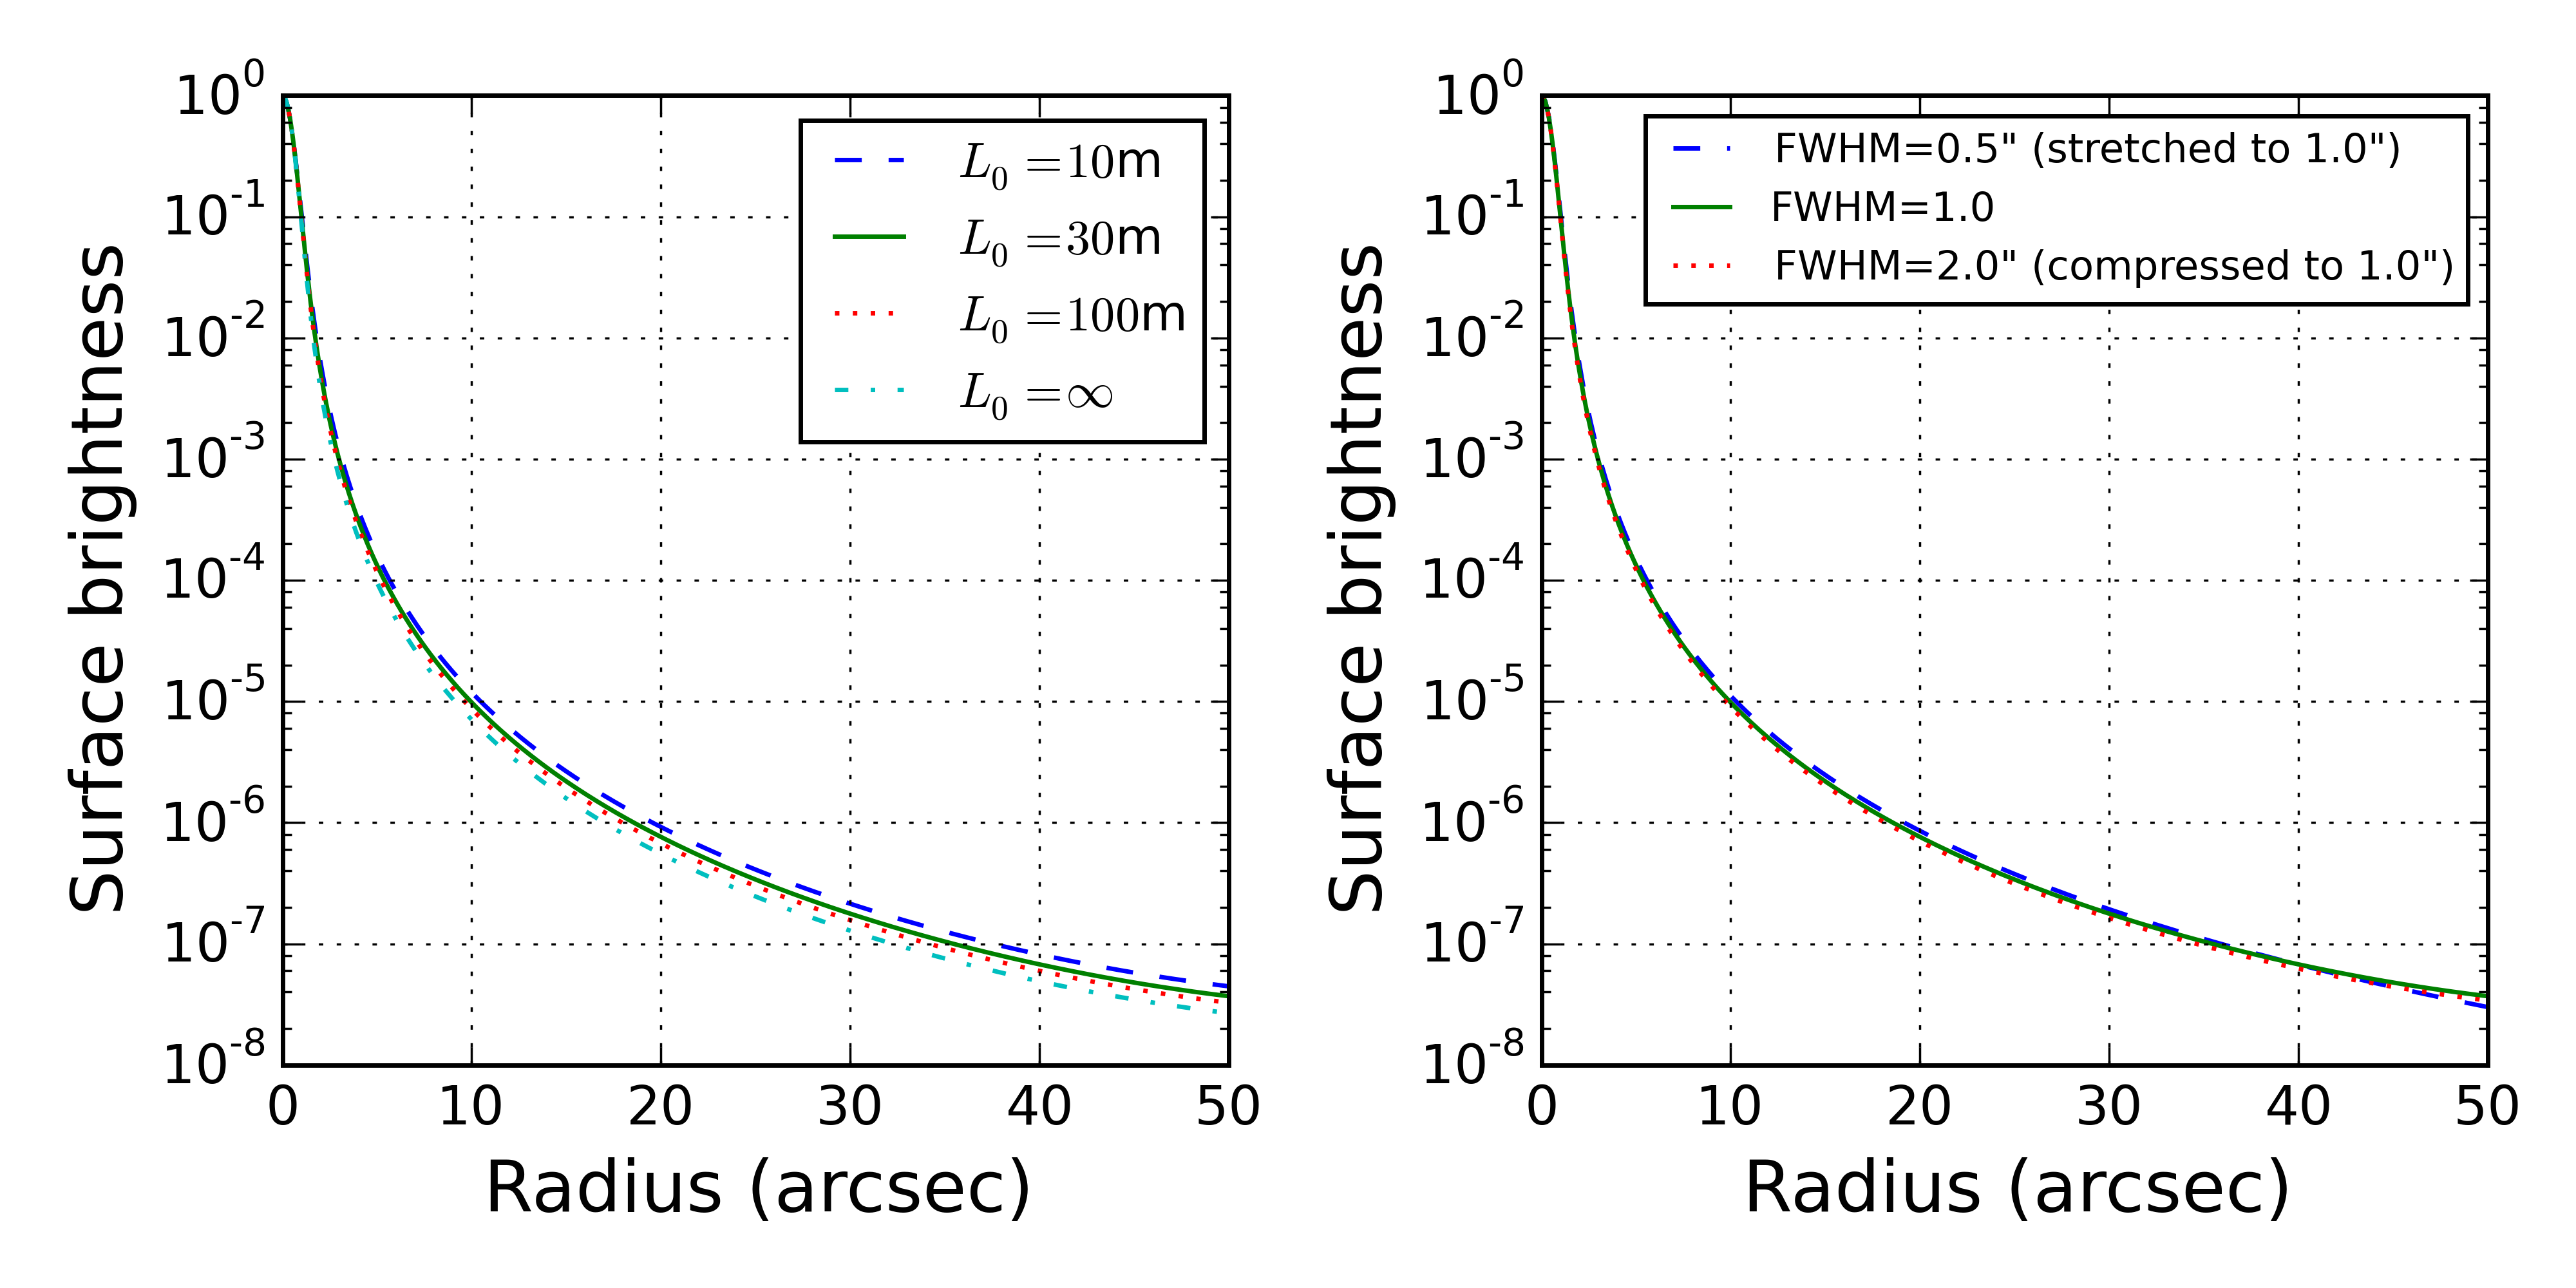
\includegraphics[width=0.8\textwidth]{FIGURES/vonK.png}
\vskip -0.2in 
\caption{PSF radial profiles with the \vk~model for a few different
  outer scale ($L_0$) values (left) and $r_0$ values (right). 
All profiles have FWHM of 1.0 arcsec, and
  are normalized to unit peak intensity. The \vk~model becomes
  Kolmogorov when $L_0 = \infty$.
In the right plot, the dashed and dotted profiles are created with
$L_0 = 30$m, and 
FWHM of 0.5 arcsec and 2.0 arcsec, respectively, then stretched and compressed to 1.0 arcsec.
\label{fig:vonK}}
\end{figure}

The $\chi^2$ is defined using the first four data points on the
measured radial profiles, at 0.16, 0.51, 0.87 and 1.44 arcsec,
respectively. These points correspond to highest photon counts, and 
also are least susceptible to errors in the background brightness
estimates. 
The error estimates on these data points come from the original SDSS measurements.

Although the fitted
curves agree with the input data points very well, generally much better than the
original 6-parameter double-Gaussian fit by SDSS, they do not always describe
the PSF tail beyond $\sim 15$ arcsec radius. 
Some examples of such fits are shown in Fig.~\ref{fig:psffit}.
This discrepancy is easily understood
because the PSF tails in the optical bands can be 
different due to the properties of the CCDs.
The SDSS $u$-, $g$-, $r$-, and $z$-bands differ only slightly due to
changing conversion depth. It is known that the $i$-band PSF has ``stronger tails''
because of scattering in the CCD.  The Si is transparent at long $i$-band wavelengths 
so light goes all the way through the chip and is reflected off the solder, and passes 
back up through the Si. This effect is not visible in the $z$-band because in this case
thick front-side illuminated chips are used (in all other bands, thin back-side chips are used). 



\subsection{Instrumental PSF \label{sec:instrPSF}} 

To improve the fit quality at large radii, in the second fitting step we introduce an
empirical ``instrumental'' PSF. Despite the name, this component might also include 
effects not modeled by the \vk~theory, such as aerosol scattering in the atmosphere,
dust on the mirrors, and scattering in the CCDs. The observed PSF can be expressed 
as a convolution of the atmosphere, represented 
by the \vk, and the instrumental PSF,
\begin{equation}
        \textrm{PSF} = \textrm{vonK} (\textrm{FWHM}) \otimes
        \textrm{PSF}_{\textrm{inst}},
\label{eq:conv}
\end{equation} 
where vonK is the \vk~shape, whose only parameter, FWHM, is fixed to
the value from step one.
Fig.~\ref{fig:psffit} shows that the tails of the PSF can be well
described using a second order polynomial in the logarithmic space of
the intensity.
Meanwhile, since $\textrm{PSF}_{\textrm{inst}}$ is a convolution
kernel, we can use a narrow Gaussian to describe its central core.
We define the functional form of the instrumental PSF as
\begin{equation}
        \textrm{PSF}_{\textrm{inst}} = \exp(-\frac{r^2}{2\sigma^2}) + 10^p,
\label{eq:psfinst}
\end{equation} 
where $p$ is a second order polynomial.
The standard deviation of the Gaussian, $\sigma$, cannot be
too wide because the \vk~term already well describes the core of the
PSF.
We found that $\sigma = 0.1$ arcsec is an acceptable choice.

We define the second order polynomial $p$ as
\begin{equation}
        p = \eta(ar^2+br+1).
\label{eq:psfinstp}
\end{equation} 
Because the shape of the instrumental PSF tail should not vary with
time, but does vary with the filter and camera column,
we determine the values of $a$ and $b$ for each band-camera-column
combination using one representative
field, then fix them at those values for all step-two fits.
For each SDSS PSF radial profile,
these one-time least-square fits use all the data points with radii up
to $\sim$30 arcsec.
Each fit has $a$, $b$, and $\eta$ as free parameters, and involves a 2-dimensional convolution (see Eq.~\ref{eq:conv}),
The fits are very slow but need to be done only once.
We used here run 94, field 11 for these one-time fits, but verified that 
the results are stable for other choices of run and field. 
The best-fit values of $a$ and $b$ are listed in Table~\ref{tab:abc}.

For step-two PSF fitting, parameters $a$ and $b$ are
fixed for each band-camera-column combination.
$\eta$, the relative normalization of the instrumental PSF
tail in the logarithm-space, is the only free
parameter.
This second fitting step is also a least-square fit with a
2-dimensional convolution, using all the data points
with radii up to $\sim$30 arcsec.
Each two-step PSF fit can be done in a few seconds.
Fig.~\ref{fig:psffit} shows the results of our PSF fits from run 4874. The two-parameter
fits describe the PSF radial profiles quite well, both in the core and
in the tails. The addition of the instrumental PSF 
(dot-dashed lines in Fig.~\ref{fig:psffit})
significantly improves the fit quality, 
especially in the $i$-band. 

Fig.~\ref{fig:psffit} also shows the original SDSS ``double Gaussian plus power-law wing'' fits,
described by Eq.~\ref{eq:SDSSPSF}. They sometimes fail catastrophically; our analysis revealed
two kinds of failures: one case is characterized by $p_0 =10^{-7}$ and
another by $\beta$=3 or 10.
For the sample of 947,400 PSF fits analyzed here, each failure case occurs with a frequency of about 12\%. 
Inspection of the SDSS code (findPsf.c) reveals that these values signal bad fits which did not 
converge for various (unknown) reasons. 

There are a total of 108 runs in the SDSS Stripe 82 dataset. Among them, run 4874 is the longest, 
with 981 fields. In the rest of this paper, whenever we illustrate results from a single run, 
we always use run 4874 as the fiducial example run. 


\begin{figure}[th]
\centering
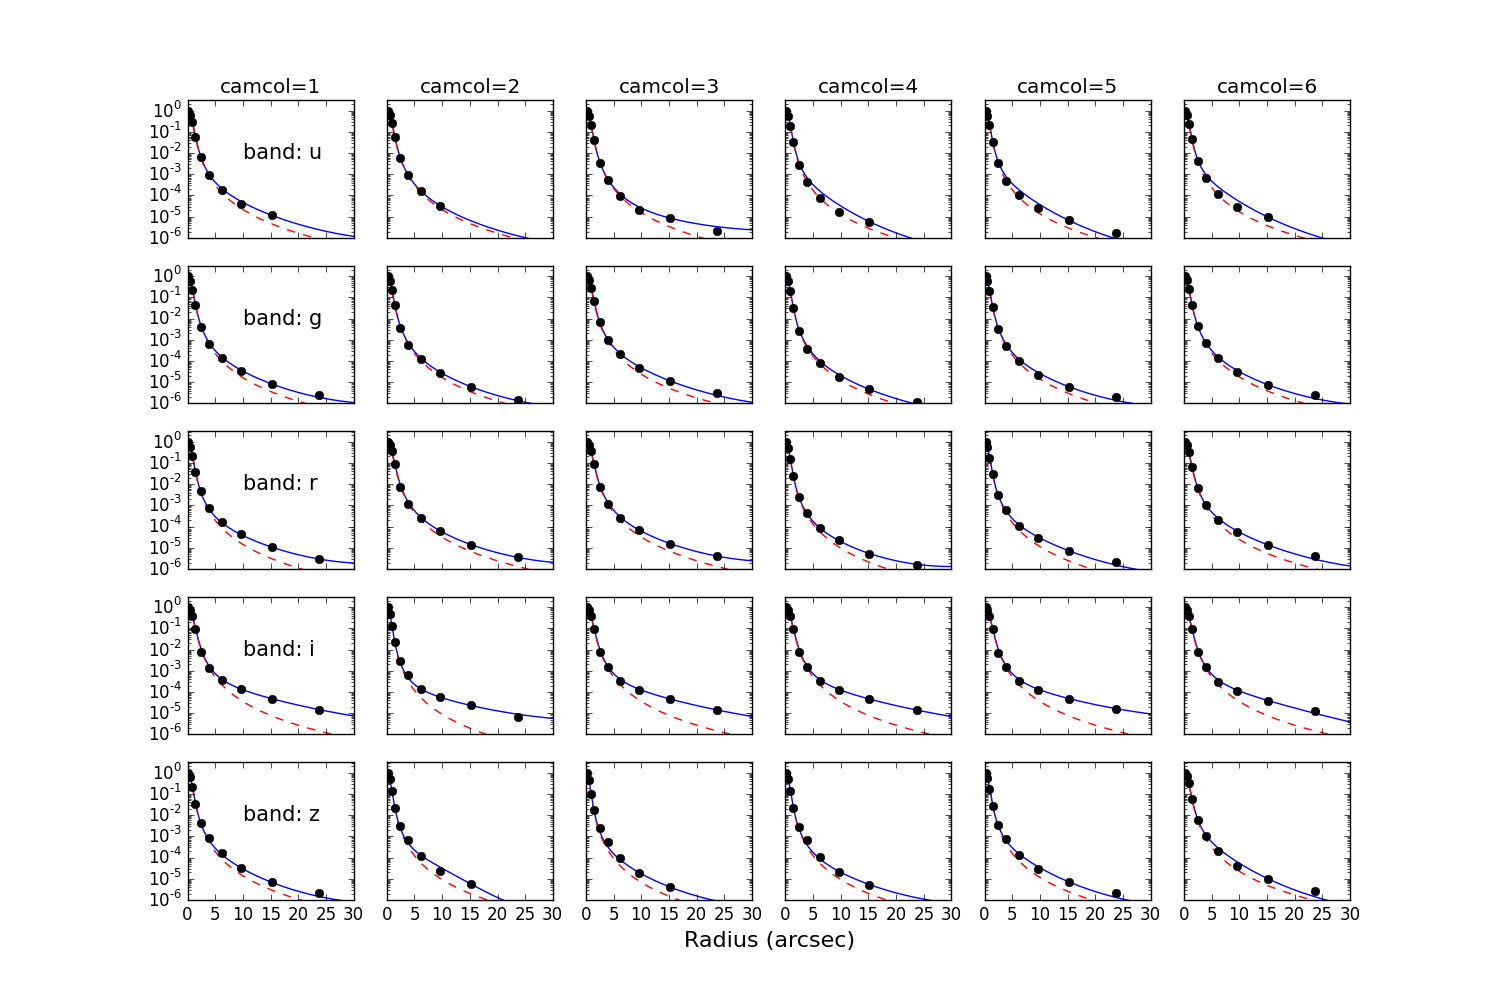
\includegraphics[width=1.0\textwidth]{FIGURES/psffit.png}
\vskip -0.3in
\caption{Fits to the PSF radial profiles from run 4874, field 121. Symbols are SDSS data. 
  Red dashed curves are the best one-parameter \vk~fits. Black solid curves are the red
  curve convolved with the instrumental PSF (green dot-dashed lines), where the scaling factor
  (relative normalization) 
  for the tail component is allowed to vary. 
As a reference, the original ``SDSS double Gaussian plus power-law wing'' fits,
described by eq.~\ref{eq:SDSSPSF}, 
 are shown in blue dotted lines -- they sometimes fail catastrophically (see text). 
Note that the y-axis is shown on the logarithmic scale.
\label{fig:psffit}}
\end{figure}


\begin{table}[th]
\begin{center}
\caption{Values for instrumental PSF shape parameters $a$ and $b$.\label{tab:abc}}
\begin{tabular}{c|c|rrrrrr}
\tableline\tableline
\multicolumn{2}{c|}{} & \multicolumn{6}{c}{Camera Column} \\\cline{3-8}
\multicolumn{2}{c|}{} & 1 & 2 & 3 & 4 & 5 & 6\\\hline
   & a($\times 10^{-4}$) & $-$4.4 & $-$4.4 & $-$1.9 & $-$4.4 & $-$4.4& $-$4.4\\
 $u$& b($\times 10^{-2}$) & 3.3   & 3.3       & 1.3       &      4.7 &4.7   & 4.7\\ \hline
  & a($\times 10^{-4}$) & $-$5.3 & $-$5.3 & $-$4.4 & $-$4.4 & $-$5.3&$-$5.3 \\
 $g$& b($\times 10^{-2}$) & 3.5  & 3.5      & 3.3       &        3.3 &3.5 & 3.5\\\hline
  & a($\times 10^{-4}$) & $-$4.9 & $-$4.9 & $-$4.9 & $-$5.8 &$-$4.4 & $-$4.4\\
 $r$& b($\times 10^{-2}$) & 3.1 & 3.1         & 3.1     &        3.3 &3.3 & 3.3\\\hline
  & a($\times 10^{-4}$) & $-$1.3 & $-$2.2& $-$1.3 & $-$1.3 & $-$1.8& -0.4\\
 $i$& b($\times 10^{-2}$) & 1.7 & 1.8        & 1.7      &        1.7 &1.7 & 1.5\\\hline
  & a($\times 10^{-4}$) & $-$6.2 & 4.4     & $-$6.2 & $-$4.4  &$-$6.2 & $-$4.4\\
 $z$& b($\times 10^{-2}$) & 4.0 & 2.0      & 4.0      &        3.1 &4.4 & 4.7\\
\tableline
\end{tabular}
\end{center}
\end{table}
